\chapter{Experimentele analyse}\label{Experiment}

Nu we alle achterliggende theorie van het experiment in hoofdstuk \ref{Lectuur} gezien hebben, kunnen we van start gaan. 

Om te weten of er technieken voor Engelse gevoelsanalyse gelijk toepasbaar zijn op het Nederlands en te achterhalen wat juist deze verschillen zijn, hebben we het onderzoek in drie experimenten opgesplitst. De gevoelsanalyse voor deze experimenten bestaat er telkens uit om te bepalen of de gegeven tekst een positive of negatieve emotie uitdrukt. Als eerste experiment vergelijken we de prestaties van de eerder besproken technieken in hoofdstuk \ref{Lectuur} op het Engels met die van het Nederlands. Vervolgens hopen we nog iets meer inzicht te krijgen in de verschillen door een classificatie uit te voeren op basis van Engels en Nederlands geannoteerde woordenlijsten van gevoelens. Als laatste gaan we nog iets dieper in op de Nederlandse gevoelsanalyse en kijken we hoe deze zich gedraagt op data met verschillende onderwerpen.

Voor dat we kunnen beginnen aan de experiment, moeten we eerst over een dataset beschikken waarmee we de algoritmes kunnen trainen en testen. In \ref{De Dataset} gaan we dieper op de dataset. Uiteindelijk is het beschikken over een goede dataset even belangrijk als het beschikken over goede technieken voor dit experiment. 

% Het doel van het experiment is aan de hand van enkele algemene technieken uit te Machine Learning een gevoelsanalyse uitvoeren op Nederlandse tekst, waarbij een algoritme het onderscheid aanleert tussen positief negatief. Het doel is om een algoritme te bekomen dat kan bepalen of een tekst een positieve of negatieve emotie uitdrukt. De prestatie van zo'n algoritme wordt in dit experiment beoordeeld op basis van de classificatieprecisie.  Wanneer het algoritme met een hoge precisie classificeert en bijna alle input correct kan classificeren als positief of negatief, dan spreken we van een goede prestatie. Wanneer de classificatieprecisie rond de 50\% of minder ligt, spreekt men van een slechte prestatie. Een classificatieprecisie van 50\% kan men vergelijken met een classificatiealgoritme dat telkens bij het bepalen van de output een munt gaat opgooien en op basis van kop of munt de output gaat bepalen. Wat neerkomt op het at random bepalen van de output.\\
% %
% Vooraleerst we de resultaten van het experiment bekijken, hebben we het in \ref{De Dataset} over de dataset die we gebruiken. Er is gekozen om gevoelsanalyse uit te voeren op film-, boek- en muziekrecensies. Waarom er is voor gekozen en hoe het verzamelen van de data is verlopen, wordt uitgelegd in deze sectie. In \ref{Naive Bayes Classifier met hetzelfde onderwerp voor trainings- en testset} en \ref{Naive Bayes Classifier met verschillend onderwerp voor trainings- en testset} volgen dan de experimenten en als laatste vatten we alle de bevindingen van het experiment samen in \ref{Conclusie experiment}.

\section{De Dataset}\label{De Dataset}

Als data voor het experiment is er gekozen voor gebruikersrecensies, meer bepaald film-, muziek- en boekrecensies. Recensies bieden alles wat we nodig hebben. Een recensie drukt of wel positieve, negatieve of neutrale mening uit. Maar omdat er meestal een rating aanwezig is bij de review, is het gemakkelijk om de data automatisch te labelen en enkel de positieve en negatieve reviews op te nemen in onze dataset. Verder door het grote aanbod aan reviewsites is het aanbod aan film-, boek- en muziekrecensies enorm en maakt het gebruik van gebruikersrecensies de recensies nog eens toegankelijk en niet te specifiek. 

Voor deze experimenten is de dataset met Engelse filmrecensies afkomstig van een eerder onderzoek door \cite{maas-EtAl:2011:ACL-HLT2011}. De recensies deze website zijn afkomstig van \url{http://www.imdb.com/} en zijn eveneens afkomstig van gebruikers. Voor de Nederlandse reviews waren er geen datasets beschikbaar en moesten deze gescraped worden. De websites \url{moviemeter.nl}, \url{boekmeter.nl} en \url{muziekmeter.nl} vormde de perfecte bron aan informatie om te scrapen. Ze bevatten allemaal toplijsten met films, boeken of muziekalbums waarop vele gebruikers hun persoonlijke mening plaatsen. Verder was er bij iedere recensie duidelijk een score aanwezig, die het mogelijk maakte om de recensies automatische te labelen. Belangrijk om te vermelden is dat zowel bij het labelen van de Engelse als de Nederlandse dataset dezelfde voorwaarden werd gerespecteerd. Enkel hoog gepolariseerde recensies werden beschouwd in de dataset. Onderzoek rond polarisatie classificatie (\cite{maas-EtAl:2011:ACL-HLT2011}) ondersteund deze keuze. Een recensie werd negatief gelabeld als het een score had van 4 op 10 of minder. Een positieve labeling werd gegeven aan recensies met een score van 6 op 10 of meer.\\

\begin{figure}[h]%
    \centering
    \subfloat{{
\includegraphics[width=10cm]{voorbeeldrecensie} }}%
    \caption{Een voorbeeld van een positieve commentaar op \url{moviemeter.nl}}%
\end{figure}
\newline

Alle Nederlandse recensies zijn afkomstig van de ``All Time Top 250''-toplijst op de betreffende website. Onderstaande linkertabel geeft het aantal verzamelde Nederlandse recensies van ieder onderwerp weer, waarbij een onderscheid wordt gemaakt tussen positief en negatief. Analoog wordt dit in de rechtertabel voor de Engelse recensies weergegeven.\\

\begin{table}[h]
\centering
\setlength\tabcolsep{2pt}
\begin{minipage}[t]{0.48\textwidth}
\centering
\begin{tabular}{l|l|l|}
\cline{2-3}
                                      & Positief & Negatief \\ \hline
\multicolumn{1}{|l|}{Filmrecensies}   & 197358   & 17978    \\ \hline
\multicolumn{1}{|l|}{Muziekrecensies} & 15197    & 3019     \\ \hline
\multicolumn{1}{|l|}{Boekrecensies}   & 146      & 3719     \\ \hline
\end{tabular}
\caption{Aantal verzamelde Nederlandse recensies} 
\end{minipage}%
\hfill
\begin{minipage}[t]{0.48\textwidth}
\centering
\begin{tabular}{l|l|l|}
\cline{2-3}
                            & Positief & Negatief \\ \hline
\multicolumn{1}{|l|}{Films} & 197358   & 17978    \\ \hline
\end{tabular}
\caption{Aantal verzamelde Engelse recensies}
\end{minipage}
\end{table}


Om nog een beter inzicht te krijgen over de dataset geven onderstaande tabellen nog wat extra statistieken weer over de datasets.\\

\begin{table}[h]
\centering
\setlength\tabcolsep{2pt}
\begin{minipage}[t]{0.48\textwidth}
\centering
\begin{tabular}{l|l|l|}
\cline{2-3}
                & Positief & negatief \\ \hline
\multicolumn{1}{|l|}{Filmrecensies}   & 60       & 75       \\ \hline
\multicolumn{1}{|l|}{Muziekrecensies} & 89       & 105      \\ \hline
\multicolumn{1}{|l|}{Boekrecensies}   & 58       & 61    \\ \hline   
\end{tabular}

\caption{Gemiddeld aantal woorden voor een Nederlandse recensie} 
\end{minipage}%
\hfill
\begin{minipage}[t]{0.48\textwidth}
\centering
\begin{tabular}{l|l|l|}
\cline{2-3}
                                   & Positief & Negatief \\ \hline
\multicolumn{1}{|l|}{Filmrecensie} & 229      & 228      \\ \hline
\end{tabular}
\caption{Gemiddeld aantal woorden voor een Engelse recensie}
\end{minipage}
\end{table}

\begin{table}[h]
\centering
\setlength\tabcolsep{2pt}
\begin{minipage}[t]{0.48\textwidth}
\centering
\begin{tabular}{l|l|l|}
\cline{2-3}
                                      & Positief & Negatief \\ \hline
\multicolumn{1}{|l|}{Filmrecensies}   & 2,64\%   & 7,41\%   \\ \hline
\multicolumn{1}{|l|}{Muziekrecensies} & 7,44\%   & 12,52\%  \\ \hline
\multicolumn{1}{|l|}{Boekrecensies}   & 10,29\%  & 25,39\%  \\ \hline
\end{tabular}

\caption{Percentage woorden van het totaal aantal woorden in de Nederlandse dataset dat uniek is.} 
\end{minipage}%
\hfill
\begin{minipage}[t]{0.48\textwidth}
\centering
\begin{tabular}{l|l|l|}
\cline{2-3}
                                    & Positief & Negatief \\ \hline
\multicolumn{1}{|l|}{Filmrecensies} & 4,39\%   & 4,41\%   \\ \hline
\end{tabular}
\caption{Percentage woorden van het totaal aantal woorden in de Engelse dataset dat uniek is.} 
\end{minipage}
\end{table}

\newpage
\begin{figure}%
    \centering
    \subfloat{{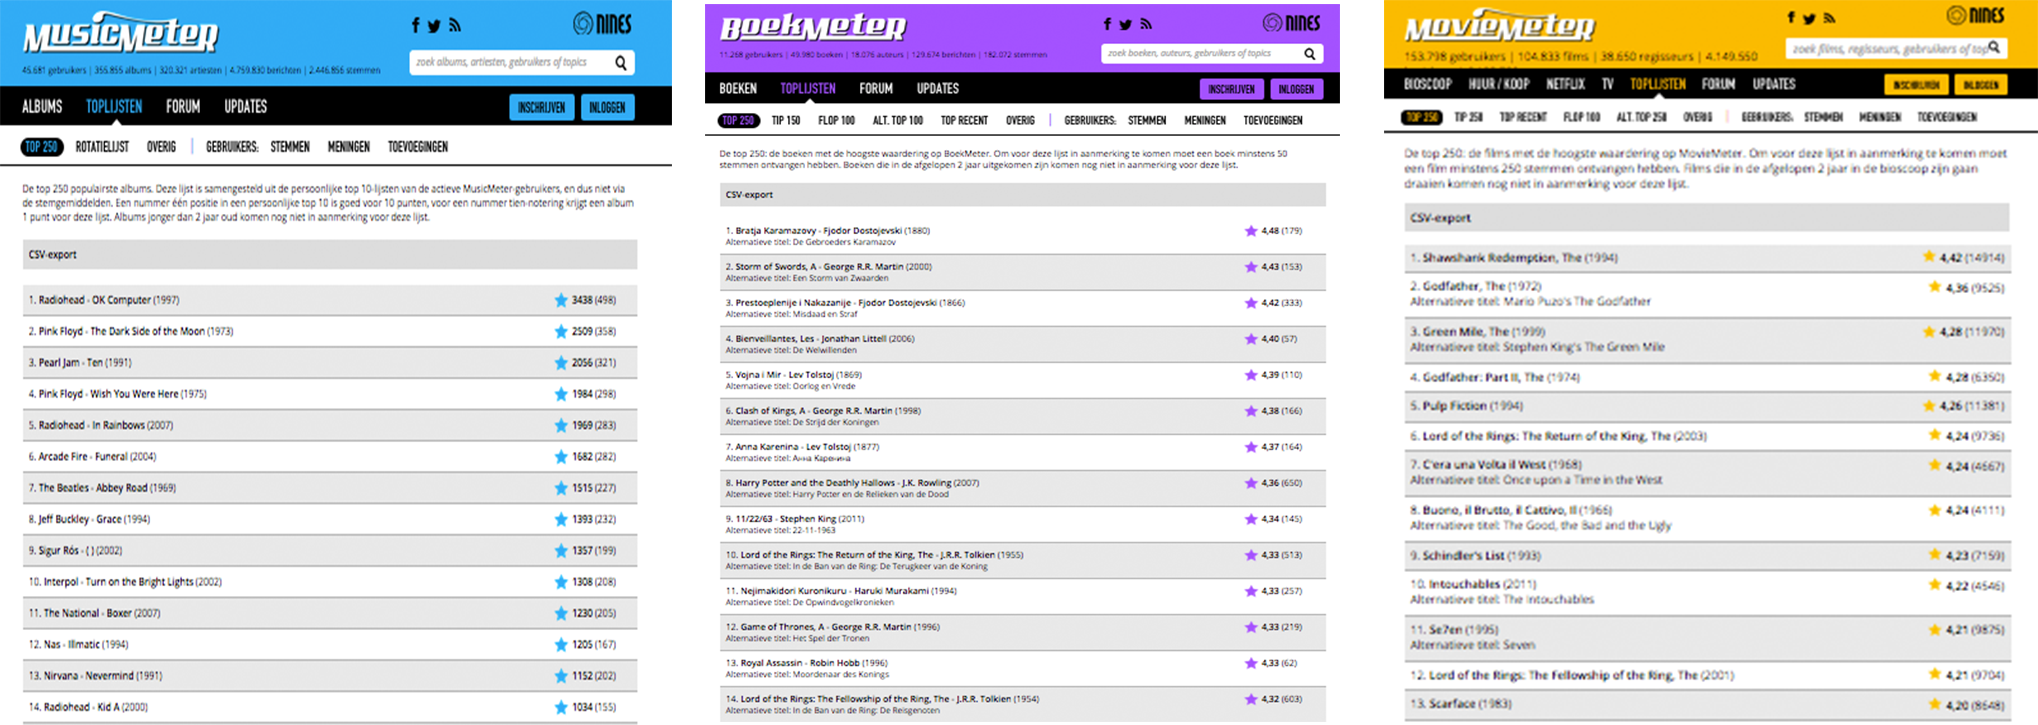
\includegraphics[width=15cm]{toplijsten} }}%
    \caption{de ``All Time Top 250''-toplijsten op de websites}%
\end{figure}


Voor het tweede experiment hebben we als woordenlijsten het \textit{Opinion lexicon} gebruikt, dat voor het eerst werd samengesteld door \cite{hu2004mining}. De woordenlijsten bestaan uit een lijst met negatieve en een lijst met positieve woorden. De lijsten bevatten in totaal ongeveer 6800 woorden en zijn enkel in het Engels verkrijgbaar. De Nederlandse woordenlijsten hebben we verkregen door de Engelse lijsten te vertalen met behulp van Google vertalen.\\

Onderstaande tabel geeft weer hoe de woordenlijsten zich tegenover elkaar verhouden.

\begin{table}[]
\centering
\caption{Aantal woorden in iedere woordenlijst}
\label{my-label}
\begin{tabular}{l|l|l|}
\cline{2-3}
 & Positief & Negatief \\ \hline
\multicolumn{1}{|l|}{Engels Woordenlijsten}     & 2006     & 4783     \\ \hline
\multicolumn{1}{|l|}{Nederlands Woordenlijsten} & 2006     & 4647     \\ \hline
\end{tabular}
\end{table}

\section{Engelse gevoelsanalyse versus Nederlandse Gevoelsanalyse}\label{Engelse gevoelsanalyse versus Nederlandse Gevoelsanalyse}
Als eerste experiment vergelijken we Engelse gevoelsanalyse met die van Nederlandse gevoelsanalyse. Concreter gaan we de geziene technieken in  hoofdstuk \ref{Lectuur} gebruiken om filmrecensies naar positieve en negatieve recensies te classificeren en vergelijken we deze prestaties voor het Engels en het Nederlands. De prestatie wordt bepaald op basis van de precisie waarmee de classifier de recensies classificeert. De precisie die we opnemen voor een classifier wordt bepaald door het gemiddelde te nemen van 30 runs. Bij iedere run wordt er een ongetrainde classifier getraind met een trainingsset en wordt de precisie getest door het classificeren van de testset. In dit experiment bestaat iedere trainingsset uit 6000 samples en testset uit 2000 samples. Ook zijn ze telkens willekeurig samengesteld en gebalanceerd. Dit wil zeggen dat de datasets telkens voor de helft uit positieve en de andere helft uit negatieve recensies bestaan en wanneer men deze willekeurig zou classificeren, men een precisie baseline van $50\%$ krijgt.\\

Voor de datasets gebruiken de besproken Engelse en Nederlandse filmrecensies uit \ref{De Dataset}.  
Onderstaande tabel geeft de belangrijkste resultaten weer van het experiment. In bijlage A vindt men de volledig tabel met resultaten.\\

\begin{table}[h]
\centering
\begin{adjustbox}{width=1\textwidth}
\begin{tabular}{|l|l|l|}
\hline
{\bf Title}                                                                         & {\bf Precisie Naive Bayes Classifier} & {\bf Precisie Decision Tree} \\ \hline
Bag of Words                                                                        & 85,74\%                               & 69,06\%                      \\ \hline
Best Feature selection on Bag of Words (max features)                               & 67,79\%                               & 69,43\%                      \\ \hline
Best Feature selection on TFIDF (max features)                                      & 74,90\%                               & 69,79\%                      \\ \hline
Bigram Collocaties                                                                  & 89,23\%                               & 69,41\%                      \\ \hline
LSA on Bag of Words (max features)                                                  & 63,11\%                               & 62,07\%                      \\ \hline
LSA on TFIDF (max features)                                                         & 78,98\%                               & 71,54\%                      \\ \hline
Term Weighting                                                                      & 86,75\%                               & 69,76\%                      \\ \hline
Verwijderen van stopwoorden                                                         & 86,62\%                               & 69,45\%                      \\ \hline
Verwijderen van stopwoorden + Best feature selection on Bag of Words (max features) & 74,43\%                               & 69,36\%                      \\ \hline
Verwijderen van stopwoorden + Best feature selection on TFIDF (max features)        & 74,94\%                               & 69,47\%                      \\ \hline
Verwijderen van stopwoorden + Bigram Collocaties                                    & 89,23\%                               & 69,51\%                      \\ \hline
Verwijderen van stopwoorden + Bigram Collocaties + Term Weighting                   & 89,29\%                               & 69,44\%                      \\ \hline
Verwijderen van stopwoorden + LSA on Bag of Words (max features)                    & 54,88\%                               & 68,66\%                      \\ \hline
Verwijderen van stopwoorden + LSA on TFIDF (max features)                           & 73,58\%                               & 75,50\%                      \\ \hline
Verwijderen van stopwoorden + Term Weighting                                        & 87,41\%                               & 69,60\%                      \\ \hline
\end{tabular}
\end{adjustbox}
\caption{Resultaten experiment op Engelse recensies}
\end{table}

\begin{table}[h]
\centering
\begin{adjustbox}{width=1\textwidth}
\begin{tabular}{|l|l|l|}
\hline
{\bf Title}                                                                          & {\bf Precisie Naive Bayes Classifier} & {\bf Precisie Decision Tree} \\ \hline
Bag of Words                                                                         & 70,51\%                               & 59,34\%                      \\ \hline
Best Feature selection Bag of Words                                                  & 58,86\%                               & 59,45\%                      \\ \hline
Best Feature selection on TFIDF ( max features)                                      & 59,53\%                               & 59,35\%                      \\ \hline
Bigram Collocaties                                                                   & 70,20\%                               & 59,35\%                      \\ \hline
LSA on Bag of Words                                                                  & 54,84\%                               & 57,53\%                      \\ \hline
LSA on TFIDF (100 features)                                                          & 63,15\%                               & 58,58\%                      \\ \hline
Term Weighting                                                                       & 69,40\%                               & 58,83\%                      \\ \hline
Verwijderen van stopwoorden                                                          & 70,35\%                               & 56,82\%                      \\ \hline
Verwijderen van stopwoorden + Best feature selection on Bag of Words ( max features) & 60,76\%                               & 56,74\%                      \\ \hline
Verwijderen van stopwoorden + Best feature selection on TFIDF (max features)         & 59,18\%                               & 56,44\%                      \\ \hline
Verwijderen van stopwoorden + Bigram Collocaties                                     & 70,63\%                               & 56,80\%                      \\ \hline
Verwijderen van stopwoorden + Bigram Collocaties + Term Weighting                    & 70,66\%                               & 56,58\%                      \\ \hline
Verwijderen van stopwoorden + LSA on Bag of Words (100 features)                     & 53,74\%                               & 57,23\%                      \\ \hline
Verwijderen van stopwoorden + LSA on TFIDF (max features)                            & 60,15\%                               & 59,24\%                      \\ \hline
Verwijderen van stopwoorden + Term Weighting                                         & 70,54\%                               & 56,55\%                      \\ \hline
\end{tabular}
\end{adjustbox}
\caption{Resultaten experiment op Nederlandse recensies}
\end{table}


Als we nu naar de resultaten kijken van het eerste experiment in \ref{Engelse gevoelsanalyse versus Nederlandse Gevoelsanalyse}, zien we dat bijna alle technieken beter presteren op de engelse dataset. Tabel XXX geeft het verschil in prestatie aan tussen het Engels en het Nederlands. We zien dat de prestatie op de Engelse dataset gemiddeld 13\% beter presteert bij de Naive Bayes Classifier en 10\% beter bij de Decision Tree.\\

\begin{table}[h]
\centering
\begin{adjustbox}{width=1\textwidth}
\begin{tabular}{|l|l|l|}
\hline
{\bf Title}                                                                          & {\bf Verschil in Precisie Naive Bayes Classifier} & {\bf Verschil in Precisie Decision Tree} \\ \hline
Bag of Words                                                                         & 14,72\%                                           & 16,05\%                                  \\ \hline
Best Feature selection Bag of Words                                                  & 8,78\%                                            & 12,18\%                                  \\ \hline
Best Feature selection on TFIDF ( max features)                                      & 15,36\%                                           & 10,44\%                                  \\ \hline
Bigram Collocaties                                                                   & 16,25\%                                           & 10,41\%                                  \\ \hline
LSA on Bag of Words                                                                  & 27,27\%                                           & 10,37\%                                  \\ \hline
LSA on TFIDF (100 features)                                                          & 19,83\%                                           & 10,69\%                                  \\ \hline
Term Weighting                                                                       & 11,79\%                                           & 10,89\%                                  \\ \hline
Verwijderen van stopwoorden                                                          & 31,79\%                                           & 11,92\%                                  \\ \hline
Verwijderen van stopwoorden + Best feature selection on Bag of Words ( max features) & 35,55\%                                           & 12,22\%                                  \\ \hline
Verwijderen van stopwoorden + Best feature selection on TFIDF (max features)         & -2,56\%                                           & 12,61\%                                  \\ \hline
Verwijderen van stopwoorden + Bigram Collocaties                                     & 18,60\%                                           & 12,61\%                                  \\ \hline
Verwijderen van stopwoorden + Bigram Collocaties + Term Weighting                    & 13,67\%                                           & 12,61\%                                  \\ \hline
Verwijderen van stopwoorden + LSA on Bag of Words (100 features)                     & 15,09\%                                           & 12,48\%                                  \\ \hline
Verwijderen van stopwoorden + LSA on TFIDF (max features)                            & -15,67\%                                          & 12,11\%                                  \\ \hline
Verwijderen van stopwoorden + Term Weighting                                         & 3,93\%                                            & 5,63\%                                   \\ \hline
{\bf Gemiddeld verschil}                                                             & {\bf 13,40\%}                                     & {\bf 10,83\%}                            \\ \hline
\end{tabular}
\end{adjustbox}
\caption{Verschil in precisie tussen het Engelse en het Nederlands (Eng - Nl)}
\end{table}

Verder zien we ook dat de prestatie voor beide talen een grotere spreiding heeft bij de Naive Bayes Classifier dan bij de Decision tree. Voor het Engels vallen de resultaten van de Naive Bayes Classifier binnen een interval van 36\% en bij de Decision Tree heeft dit interval een lengte van 14\%. Voor het Nederlandse we hetzelfde verschijnsel. De resultaten van de Naive Bayes classifier vallen binnen een interval van 18\% en bij de Decision tree is dit 2\%.\\

Als we nu als referentie de prestatie van Bag of Words nemen en kijken hoe de andere technieken presteren tegenover Bag of Words, zien we dat voor de Naive Bayes Classifier de pre-processing technieken: Bigram collocaties, Term Weighting en het verwijderen van stopwoorden positief naar voren komen. Alleen of in combinatie hebben ze een positieve invloed op de prestatie. Dit het geval voor beide talen, al is deze bevinding bij het Engels overtuigend aanwezig en bij het Nederlands eerder minimaal. Opmerkelijk is dat de combinatie van de drie pre-processing technieken bij beide talen als best presterende techniek naar boven komt. Opnieuw is bij het Nederlands dit verschil minimaal ten op zichten van de andere combinaties.\\

Voor de Decision tree springt de prestatie van /textit{Verwijderen van stopwoorden $+$ LSA + Term weighting} in het oog met 75\% als beste resultaat. Bij het Nederlands springt deze techniek er niet uit en is de prestatie zelfs minder goed als Bag of Words, al is het verschil miniem en hoort het nog steeds bij de betere resultaten van de Decision Tree.\\

Algemeen kunnen we zeggen dat de trends die we zien bij het Engels zich ook voordoen bij het Nederlands. De technieken werken ook op het Nederlands, als men weet dat in eerder onderzoek \cite{pang2002thumbs} aantoont dat een human-based classifier resultaten haalt van ongeveer 58\% tot 64\% op Engelse filmreviews, kunnen we stellen dat de technieken goede prestaties halen op Nederlandse reviews, met als de Naive Bayes Classifier de best presterende van de twee leermethoden.


\section{Classificatie op basis van geannoteerde woordenlijsten}\label{Classificatie op basis van geannoteerde woordenlijsten}


Om meer inzicht te krijgen over de verschillen in de gevoelsanalyse bij de twee talen, voeren we nog een tweede experiment uit. Bij dit experiment gaan we heel eenvoudig en intu\"itief te werk. We kijken hoe de classificatie verloopt, wannneer we enkel geannoteerde woordenlijsten met gevoelens in beschouwing nemen. Er wordt voor iedere recensie gekeken, hoeveel woorden van de recensie voorkomen in de positieve lijst en hoeveel in de negatieve. De lijst met de meest overeenkomstige woorden geeft aan of de recensie positief of negatief moet worden geclassificeerd.\\
Voor de woordenlijsten gebruiken we de eerder vermeldden woordenlijsten uit \ref{De Dataset}. De classificatie zelf testen we op de Engelse en Nederlandse filmrecensies.\\
Onderstaande tabel geeft de resultaten van de classificatie weer met als precisie het gemiddelde van 30 runs en een testset van 2000 samples random en gebalanceerd samengesteld.

\begin{table}[h]
\centering
\label{my-label}
\begin{tabular}{l|l|}
\cline{2-2}
                                           & Precisie \\ \hline
\multicolumn{1}{|l|}{Engels recensies}     & 67,43\%  \\ \hline
\multicolumn{1}{|l|}{Nederlands recensies} & 1,16\%   \\ \hline
\end{tabular}
\caption{Classificatieprecisie aan de hand van woordenlijsten}
\end{table}



Voor het tweede experiment gooiden we het over een andere boeg en werkt we met met geannoteerde woordenlijsten van gevoelens. Het resultaat voor Engelse recensies met 68\% is goed, maar voor het Nederlands met 1\% kunnen we zeggen dat de classificatie methode niet werkt. We moeten echter kritisch zijn en rekening houden met een paar dingen. Een eerste element waar we rekening mee moeten houden is de oorsprong van de woordenlijsten. De woordenlijsten zijn samengesteld op basis van Engelse recensies en  het verlies in de vertaling naar het Nederlands kan een mogelijk effect hebben op de Nederlandse classficatie. Al zien we in tabel xxx dat dit verlies beperkt wordt tot 2,5\%. Een andere invloed zijn de leenwoorden. De woorden uit de Engelse woordenlijst kunnen juist vertaald zijn door Google translate, maar kunnen onnatuurlijk overkomen in het Nederlands. Bijvoorbeeld het positieve woord \textit{cool} wordt vertaald door Google translate als \textit{koel}, wat in het Nederlands helemaal niet wordt gebruikt als positief woord. Ook de Engelse woordenschat om zich positief uit te drukken kan helemaal anders zijn dan die van het Nederlands. Als laatste heeft men ook internetslang en uitgesmeerde woorden zoals \textit{sssaaaaiiii} die niet in rekening worden gebracht. In verder onderzoek kan men dergelijke invloeden vermijden door eigenhandig een Nederlandse geannoteerde woordenlijst met gevoelens samen te stellen en deze te gebruiken voor het classificeren van de Nederlandse reviews














\section{Onderwerpgevoeligheid van Nederlandse Gevoelsanalyse}\label{Onderwerpgevoeligheid van Nederlandse Gevoelsanalyse}

Nu we weten welke methode goed presteert op het Nederlands en welke niet, kunnen we er nog iets dieper ingaan op Nederlandse gevoelsanalyse. De voorgaande experimenten zijn altijd uitgevoerd op filmrecensies en hadden goede prestaties. Het is interessant om eens te kijken of de voorgaande technieken onderwerp gevoelig zijn of niet. Concreet voor dit experiment onderzoeken we enkel de beste presterende techniek uit \ref{Engelse gevoelsanalyse versus Nederlandse Gevoelsanalyse}, namelijk de Naive Bayes Classifier in combinatie met Term weighting en het verwijderen van stopwoorden. We kijken hoe deze techniek presteert wanneer we het trainen en testen met recensies over hetzelfde onderwerp en hoe het presteert met een verschillend.  Als datasets nemen we film- , muziek en boekrecensies. De prestatie van de classifiers is telkens de gemiddelde classificatieprecisie van 30 runs, waarbij de trainingsset uit 6000 samples bestaat en de testset uit 2000 samples. 

Onderstaande kruistabel met classificatieprecisies vat de belangrijkste resultaten van het experiment samen. De volledige resultaten vindt men in bijlage B. Merk op dat men hier ook de controle op over- of onderfitting vindt. Over- en onderfitting zijn symptomen bij machine learning waarbij men de classifier over of ondertrained. Voor de volledigheid hebben we deze grafieken in de bijlage toegevoegd.    

\begin{table}[h]
\centering
\begin{tabular}{l|c|c|c|}
\cline{2-4}
                                      & \textbf{Films} & \textbf{Muziek} & \textbf{Boeken} \\ \hline
\multicolumn{1}{|l|}{\textbf{Films}} & 70,66\%         & 61,00\%         & 56,25\%         \\ \hline
\multicolumn{1}{|l|}{\textbf{Muziek}} & 62,07\%         & 82,62\%         & 56,47\%         \\ \hline
\multicolumn{1}{|l|}{\textbf{Boeken}} & 65,87\%         & 61,46\%         & 71,76\%         \\ \hline
\end{tabular}
\label{tab:alles}
\caption{Kruistabel van alle classificatieresultaten uit \ref{Naive Bayes Classifier met verschillend onderwerp voor trainings- en testset} en \ref{Naive Bayes Classifier met hetzelfde onderwerp voor trainings- en testset} met de kolommen het onderwerp van de trainingsset en de rijen het onderwerp van de testset.} 
\end{table}

Als laatste hebben nog de confusion matrixen van het experiment. Een confusion matrix geeft weer hoeveel recensies er juist en fout geclassificeerd zijn. 

\begin{table}[h]
\centering
\setlength\tabcolsep{4pt}
\begin{minipage}[t]{0.48\textwidth}
\centering
\begin{tabular}{lll}
                                 & \textbf{P}               & \textbf{N}               \\ \cline{2-3} 
\multicolumn{1}{l|}{\textbf{P'}} & \multicolumn{1}{l|}{43\%} & \multicolumn{1}{l|}{6\%} \\ \cline{2-3} 
\multicolumn{1}{l|}{\textbf{N'}} & \multicolumn{1}{l|}{18\%} & \multicolumn{1}{l|}{31\%} \\ \cline{2-3} 
\end{tabular}
\caption{Gemiddelde confusion matrix in percent voor een Naive Bayes Classifier, waar trainings- en testset over hetzelfde onderwerp gaan}
\end{minipage}%
\hfill
\begin{minipage}[t]{0.48\textwidth}
\centering
\begin{tabular}{lll}
                                 & \textbf{P}               & \textbf{N}               \\ \cline{2-3} 
\multicolumn{1}{l|}{\textbf{P'}} & \multicolumn{1}{l|}{32\%} & \multicolumn{1}{l|}{18\%} \\ \cline{2-3} 
\multicolumn{1}{l|}{\textbf{N'}} & \multicolumn{1}{l|}{21\%} & \multicolumn{1}{l|}{29\%} \\ \cline{2-3} 
\end{tabular}
\caption{Gemiddelde confusion matrix in percent voor een Naive Bayes Classifier, waar trainings- en testset over een verschillend onderwerp gaan} 
\end{minipage}
\end{table}

\begin{table}[h!]
\centering
\begin{tabular}{c >{\bfseries}r @{\hspace{0.7em}}c @{\hspace{0.4em}}c @{\hspace{0.7em}}l}
  \multirow{10}{*}{\parbox{1.1cm}{\bfseries\raggedleft eigelijke\\ waarde}} & 
    & \multicolumn{2}{c}{\bfseries voorspelde waarde} & \\
  & & \bfseries p & \bfseries n  \\
  & p$'$ & \MyBox{Waar}{Positief} & \MyBox{Vals}{Negatief}  \\[2.4em]
  & n$'$ & \MyBox{Vals}{Positief} & \MyBox{Waar}{Negatief} \\
\end{tabular}
\caption{Illustratie van de confusion matrix} 
\end{table}

